\documentclass{beamer}
\usetheme{Copenhagen}

\usepackage{siunitx}
\newcommand{\h}{\unit{\hour}}
\newcommand{\ph}{\unit{\per\hour}}
\newcommand{\um}{\unit{\micro\metre}}
\newcommand{\pums}{\unit{\per\micro\metre\squared}}
\newcommand{\nm}{\unit{\nano\mole\per\litre}}

\usepackage{amsmath}
\usepackage{amssymb}
\usepackage{cancel}
\usepackage{graphicx}
\graphicspath{{../images/}}

\title{An ODE Model of Root Zonation in \\ \emph{A. Thaliana} Mutants}
\author{Riley Wheadon}
\institute{University of British Columbia}
\date{Snacks, December 4th, 2024}

\begin{document}

\frame{\titlepage}

\begin{frame}
\frametitle{Acknowledgements}
\begin{itemize}
  \item Dr. Eric Cytrynbaum (Supervisor)
  \item Dr. Geoffrey Wasteneys (Experimental Collaborator)
  \item NSERC USRA Program
\end{itemize}
\end{frame}

\begin{frame}
\frametitle{Root Zonation}
\begin{figure}
  \centering
  \includegraphics[height=16em]{root-zonation-simple.png}
  \caption{Zonation of the root apical meristem in \emph{A. thaliana}.}
\end{figure}
\end{frame}

\begin{frame}
\frametitle{Microtubules}
\begin{figure}
  \centering
  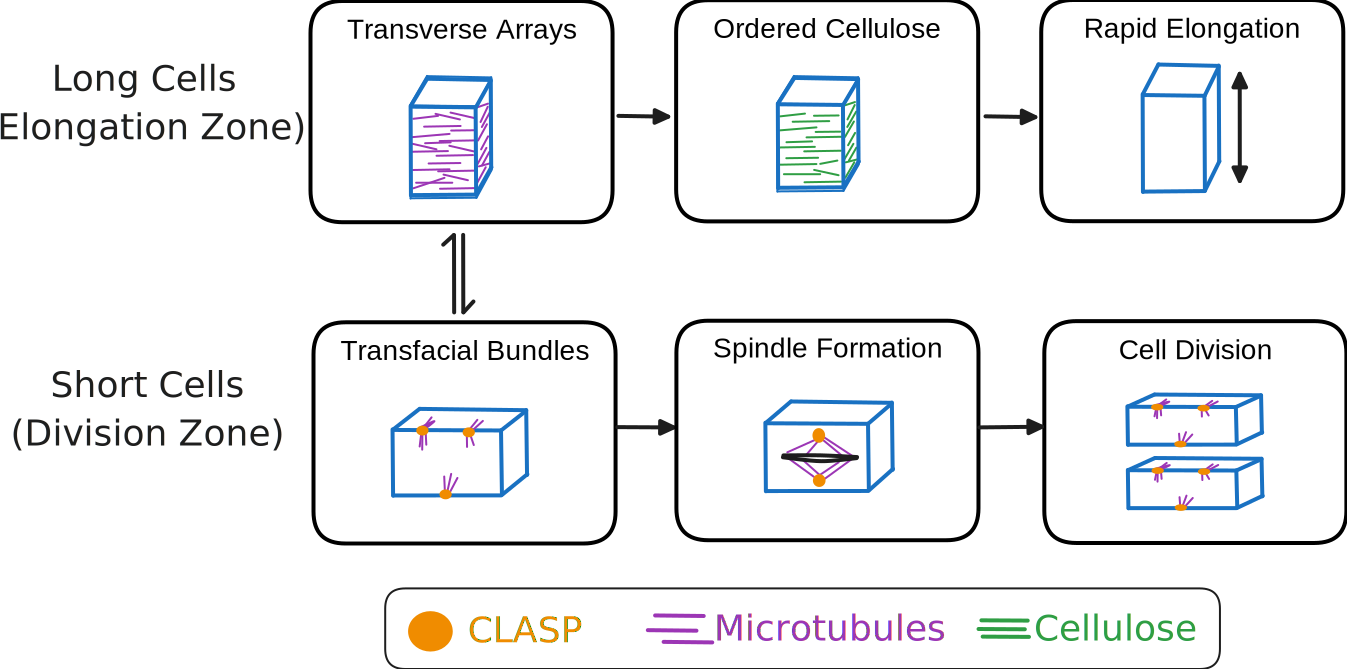
\includegraphics[width=\textwidth]{microtubule-behaviour.png}
  \caption{The arrangement of microtubules is linked with cell behaviour.}
\end{figure}
\end{frame}

\begin{frame}
\frametitle{Signalling Network}
\begin{figure}
  \centering
  \includegraphics[width=\textwidth]{network-wild-type.png}
  \caption{Hormone interactions observed in \emph{A. thaliana} roots.}
\end{figure}
\end{frame}

\begin{frame}
\frametitle{\emph{brinCLASPpro} (BRIN-CLASP) Mutant}
\begin{figure}
  \centering
  \includegraphics[width=\textwidth]{network-brin-clasp.png}
\end{figure}
\end{frame}

\begin{frame}
\frametitle{\emph{clasp-1} Mutant}
\begin{figure}
  \centering
  \includegraphics[width=\textwidth]{network-clasp-1.png}
\end{figure}
\end{frame}

\begin{frame}
\frametitle{Mutant Roots}
\begin{figure}
    \centering
    \includegraphics[height=16em]{data-binned-500.pdf}
    \caption{Experimental data from the wild type and mutants.}
\end{figure}
\end{frame}

\begin{frame}
\frametitle{Hypothesis}
\begin{figure}
    \centering
    \includegraphics[height=16em]{mutant-phenotypes.png}
    \caption{A "sizer" mechanism for division zone exit produces the different phenotypes in the wild type, BRIN-CLASP, and CLASP-1 roots!}
\end{figure}
\end{frame}


\begin{frame}
\frametitle{Growth Model Assumptions}
\begin{itemize}
    \setlength\itemsep{0.8em}
    \item We model a \emph{single column} of cells over time.
    \item Our data has no time dependence so $\Delta t$ is arbitrary.
    \item Cells grow at a basal rate $\gamma_{0}L$. 
    \item Cell growth is increased by BES1 at a rate $\gamma_{1}$. The exact model for BES1 signalling is discussed later.
\end{itemize}
\end{frame}

\begin{frame}
\frametitle{Division Model Assumptions}
\begin{itemize}
    \setlength\itemsep{0.8em}
    \item Cells complete a cell cycle and divide when $D=1$.
    \item Cells also must be at least $m\,\um$ long to divide.
    \item Cell division creates two cells with length $L / 2$ and $D = 0$.
    \item Progress in the cell cyle proceeds at a basal rate $d_{0}$.
    \item Progress in the cell cyle is inhibited by \emph{length}. 
\end{itemize}
\medskip
\end{frame}

\begin{frame}
\frametitle{Abridged Signalling Network}
\begin{figure}
  \centering
  \includegraphics[width=\textwidth]{network-simplified.png}
  \caption{Simplified signalling network used in the model.}
\end{figure}
\end{frame}


\begin{frame}
\frametitle{Equations}

The intracellular equations are assumed to be in QSS:
$$
\begin{aligned}
  0 &= \frac{ dC }{ dt } = (c_{0} - c_{1}R_{B}) - c_{2}C \\[5pt]
  0 &= \frac{ dR_{T} }{ dt } = (r_{0}  + r_{1}C) - r_{2}R_{T} \\[5pt]
  0 &= \frac{ dR_{B} }{ dt } = k_{\text{on}}(R_{T} - R_{B})B_{\text{free}} - k_{\text{off}}R_{B} \\[5pt]
\end{aligned} 
$$

Growth and division take place on a much longer time scale:
$$
\begin{aligned}
\frac{ dD }{ dt } &= (1 + \delta_{0}C) \left( 1 - \frac{ L^{ n } }{ \delta_{1}^{ n } + L^{ n } } \right)  \\[5pt]
\frac{ dL }{ dt } &= \left(\gamma_{0}  +  \gamma_{1}R_{B}\right)L  
\end{aligned}
$$
\end{frame}

\begin{frame}
\frametitle{Initial Results}
\begin{figure}
  \centering
  \includegraphics[height=16em]{column-original-fit.pdf}
  \caption{The model failed to differentiate cell lengths in the BRIN-CLASP mutant from the wild type.}
\end{figure}
\end{frame}

\begin{frame}
\frametitle{Troubleshooting the Model}
The BRIN-CLASP mutant is behaving almost identically to the wild type. There are two possible ways to rescue the mutant:
\begin{enumerate}
  \item Make cells in the BRIN-CLASP mutant \textbf{grow faster}.
  \item Make cells in the BRIN-CLASP mutant \textbf{divide slower} relative to the wild type, which makes them larger on average.
\end{enumerate}
\end{frame}

\begin{frame}
\frametitle{Solution 1: Promoting Growth in BRIN-CLASP}
\onslide<1->{\textbf{Why?} The BRIN-CLASP mutant has more CLASP and thus more BRI1 receptors. These additional receptors could be binding to brassinosteroid molecules that weren't included in our model, increasing BES1 signalling and growth.}

\bigskip

\onslide<2->{\textbf{How?} Increase the level of extracellular BL to account for other brassinsteroids. This (as well as some other changes) ultimately \emph{did not} rescue the BRIN-CLASP mutant.}
\end{frame}

\begin{frame}
\frametitle{Solution 2: Inhibiting Division in BRIN-CLASP}
\onslide<1->{\textbf{Why?} The higher concentration of CLASP in the BRIN-CLASP mutant increases the amount of transfacial microtubule bundles. An excess of these bundles could prevent tubulin from forming the mitotic spindle.}

\bigskip

\onslide<2->{\textbf{How?} To implement this change, we modify the division equation to lower the division rate for low \emph{and} high CLASP concentrations.
$$
\frac{ dD }{ dt } = (\color{red}\sigma_{0} + \sigma_{1}C - C^{2}\color{black})\left(1 - \frac{ L^{ n } }{ \delta_{1}^{ n } + L^{ n } }\right)
$$}
 
\end{frame}

\begin{frame}
\frametitle{Updated Results (1)}
\begin{figure}
  \centering
  \includegraphics[height=16em]{column-modified-fit.pdf}
  \caption{The updated model correctly differentiates cell lengths in the BRIN-CLASP mutant from the wild type.}
\end{figure}
\end{frame}

\begin{frame}
\frametitle{Updated Results (2)}
The updated model accurately explains the mutant phenotypes:
\begin{center}
\medskip
\begin{tabular}{|c c c c |} 
 \hline
 Mutant & Length & Division Zone Size & Divisions  \\ [0.5ex] 
 \hline
 Wild Type & $43\,692\um$ &  $456.5\um$ & $324$ \\ 
 \hline
 BRIN-CLASP & $28\,352\um$ &  $275.0\um$ & $213$ \\
 \hline
 \emph{clasp-1} & $19\,241\um$ &  $234.5\um$ & $142$ \\
 \hline
\end{tabular}
\end{center}
\end{frame}

\begin{frame}
\frametitle{Conclusion}

\onslide<1->{\textbf{Key Idea}: A mechanism which causes the CLASP protein to inhibit cell division at superphysiological concentrations is sufficient to explain the BRIN-CLASP mutant (and \emph{clasp-1} and wild type).}

\bigskip

\onslide<2->{\textbf{Next Steps:}}
\begin{itemize}
 \item<2-> Preparing the results presented today for publication.
 \item<2-> Exploring other mechanisms for zonation (i.e. "timer").
 \item<2-> Integrating this work with intracellular microtubule models.
 \item<2-> Modelling the effects of CLASP on auxin signalling.
\end{itemize}

\bigskip

\onslide<3->{Thanks for listening. Any questions?}

\end{frame}

\end{document}


